\subsection{Interfaces}
\subsubsection{Syntax}
\begin{lstlisting}[style=Csharp]
  public interface IList: Icollection, IEnumerable
  {
    int Add (object value);             //methods
    bool Contains(object value);        
    ...
    bool isReadOnly{get;}               //Property
    ...
    object this [int index]{get; set;}  //Indexer
    
  }
\end{lstlisting}
\begin{itemize}
  \item Ein Interface ist eine pure abstrakte Klasse $\rightarrow$ Nur
  Signaturen, keine Implementationen
  \item Kann Methoden, Properties, Indexers und Events enthalten
  \item Kann \textbf{nicht} Felder, Konstanten, Konstruktoren, Destruktoren,
  Operatoren oder nested Types enthalten. 
  \item Interface Members sind implizit public abstract (virtual)
  \item Interface Members dürfen nicht statisch sein
  \item Klassen und Structs können mehrere Interfaces implementieren. 
  \item Interfaces können von anderen Interfaces erben
\end{itemize}

\subsubsection{Implementierung durch Klassen und Structs}
\begin{lstlisting}[style=Csharp]
  class MyClass: MyBaseLcass, IList, ISerializable
  {
    public int Add (object value){...}
    public bool Contain (object value){...}
    ...
    public bool IsReadOnly {get {...}}
    ...
    public object this [int index] {get{...} set{...}}
  }
\end{lstlisting}
\begin{itemize}
	\item Eine Klasse kann von einer einzelnen Basisklasse erben, kann aber mehrere
	      Interfaces implementieren. Ein Struct kann nicht von einem Type erben, aber
	      mehrere Interfaces implementieren. 
	\item Jeder Interfacemember (Methode, Property, Indexer) muss aus einer
	      Basisklasse implementiert oder vererbt sein. 
	\item Implementierte Interfacemethoden müssen \textbf{nicht} mit override
	      deklariert werden. 
	\item Implementierte Interfacemethoden können als abstract deklariert werden.
	      (Ein interface kann also aus einer abstrakten Klasse implementiert werden)
	\item Soll eine Funktion z.B Add() in einer abgeleiteten Klasse von MyClass überschrieben werden,
	      muss sie mit \textbf{virtual} deklariert werden (obwohl Add() schon implizit virtual ist in IList).
\end{itemize}

\begin{multicols}{2}
\subsubsection{Working with Interfaces}
\begin{lstlisting}[style=Csharp]
  //Zuweisungen: 
  MyClass c = new MyClass(); 
  IList list = c; 
  
  //Methoden-Aufruf:
  list.Add("Tom");  //Dynamic binding -> MyClass.Add
  
  //Type check:
  if(list is MyClass)       //True
  if(list is ISerializable) //True
  
  //Type casts: 
  c = list as MyClass; 
  c = (MyClass) list; 
  ISerializable ser = (ISerializable)list;
\end{lstlisting}

\columnbreak

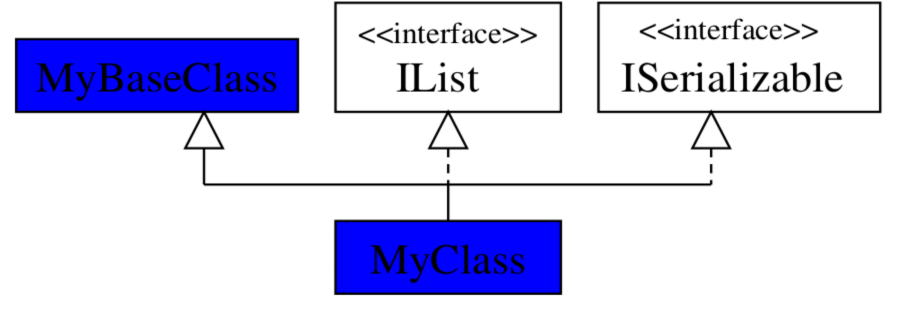
\includegraphics[width=8cm]{images/CSharp/Interface}

\end{multicols}

\begin{multicols}{2}
\subsubsection{Beispiel}
\begin{lstlisting}[style=Csharp]
  interface ISimpleReader
  {
    int Read();  
  }
  
  interface IReader:ISimpleReader
  {
    void Open(string name); 
    void Close(); 
  }
  
  class Terminal: ISimpleReader
  {
    public int Read(){...}
  }
 
 class File: IReader
 {
  public int Read(){...}
  public void Open(string name){...}
  public void Close(){...}
 }
 
 ISimpleReader sr = null; 
 sr = new Terminal(); 
 sr = new File(); 
 
 IReader r = new File(); 
 sr = r; 
\end{lstlisting}

\columnbreak

  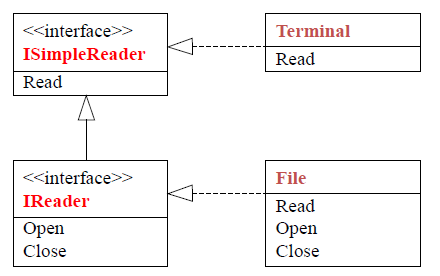
\includegraphics[height=5cm]{images/CSharp/InterfaceExample}

\end{multicols}

\subsubsection{Name Clashes}
Tritt auf wenn zwei Interfaces Methoden mit dem gleichen Namen haben.
\begin{lstlisting}
interface I1 { void F(); }
interface I2 { void F(); }

class B: I1, I2 {
	// implementation by a single F method
	public void F() { Console.WriteLine("B.F");}
	// implementation by separate F methods
	void I1.F() { Console.WriteLine("I1.F");} // Must not be public!
	void I2.F() { Console.WriteLine("I2.F");} // Must not be public!
}

B b = new B();
b.F(); // B.F

I1 i1 = b;
i1.F(); // I1.F

(b as I2).F(); // I2.F
\end{lstlisting} 